%%This is a very basic article template.
%%There is just one section and two subsections.
\documentclass[12pt,a4paper]{report}
\usepackage[ngerman]{babel}
\usepackage{amsmath,amssymb,amstext}        %Formel/Mathe Bibliotek
\usepackage[utf8]{inputenc}                 %UTF8 Codierung
\usepackage{color}                          %Farbbibliotek
\usepackage{graphicx}
\usepackage{subfig}
\usepackage{geometry}
\geometry{a4paper, top=25mm, left=40mm, right=25mm, bottom=30mm,
headsep=10mm, footskip=12mm}

\begin{document}
\tableofcontents

\section{Timing}

Um die Deltazeit zu ermitteln, müssen ein paar Berechnungen angestellt werden.
Zunächst muss das Verhältnis zum Deltawert für eine Viertelnote(PPQN) berechnet
werden. Dies wird dann mit dem Tempowert multipliziert und nochmal durch 1000
dividiert, da der Wert in Mykrosekunden angegeben ist.

\section{Musiktheorie}

Die Definition des Tons kann variieren. Für die meisten Menschen ist ein Ton
eine sinusförmige Schalldruckwelle - Sinuston. Unterscheiden lassen sich Töne in
ihrer Tonhöhe. Die Amplitude der Sinuskurve gibt die Laustärke, die
Periodendauer die Tonhöhe/Tonfrequenz in Hz an. 

Wenn man meherer Töne übereinander lagert, ergibt die ein Geräusch. Sind diese
Töne harmonisch zueinander ist das Geräusch ein Klang. Somit kann man sagen, das
ein Schalgzeug ein Geräusch erzeugt und ein Klavier einen Klang. 

Klänge haben keinen oder mehrere Obertöne, einen Grundton und keinen oder
mehrere Untertöne. Dabei nehmen Obertöne ein Vielfaches und Untertöne ein
Bruchteil der Frequenz des Grundtons ein. 

Eine Oktave besteht aus 7 Stammtönen(C, D, E, F, G, A, H) und 5 Halbtönen (Cis,
Dis, Fis, Gis, Ais).
\newpage

\section{Signalerzeugung}

Der Kammerton A ist eine Sinuston mit der Frequenz von 440 Hz und besitzt die
Notennummer 69.
Dieser Ton wird verwendet um z.B. eine Gitarre zu stimmen. Dazu nutzt
man eine Stimmgabel die nach dem Anschlagen eine Frequenz von 440 Hz erzeugt.

\begin{table}[htbp]
  \centering
  \caption{MIDI Protokoll}
    \begin{tabular}{|c|cccccccccccc|}

    \hline
    Oktave& C     & C\#   & D     & D\#   & E     & F     & F\#   & G     & G\#   & A     & A\#   & H \\
    \hline

    0     & 0     & 1     & 2     & 3     & 4     & 5     & 6     & 7     & 8     & 9     & 10    & 11 \\
    1     & 12    & 13    & 14    & 15    & 16    & 17    & 18    & 19    & 20    & 21    & 22    & 23 \\
    2     & 24    & 25    & 26    & 27    & 28    & 29    & 30    & 31    & 32    & 33    & 34    & 35 \\
    3     & 36    & 37    & 38    & 39    & 40    & 41    & 42    & 43    & 44    & 45    & 46    & 47 \\
    4     & 48    & 49    & 50    & 51    & 52    & 53    & 54    & 55    & 56    & 57    & 58    & 59 \\
    5     & 60    & 61    & 62    & 63    & 64    & 65    & 66    & 67    & 68 &\colorbox{yellow}{69}& 70    & 71 \\
    6     & 72    & 73    & 74    & 75    & 76    & 77    & 78    & 79    & 80    & 81    & 82    & 83 \\
    7     & 84    & 85    & 86    & 87    & 88    & 89    & 90    & 91    & 92    & 93    & 94    & 95 \\
    8     & 96    & 97    & 98    & 99    & 100   & 101   & 102   & 103   & 104   & 105   & 106   & 107 \\
    9     & 108   & 109   & 110   & 111   & 112   & 113   & 114   & 115   & 116   & 117   & 118   & 119 \\
    10    & 120   & 121   & 122   & 123   & 124   & 125   & 126   & 127   &       &       &       &  \\
    \hline
    \end{tabular}%
  \label{tab:addlabel}%
\end{table}%
Das MIDI Protokoll umfasst 128 Noten. Dazu muss die jeweilige Nummer in ein Ton
umgewandelt werden.

\subsection{Berechnung der Frequenz}

Ausgehend davon das der Ton A mit seiner Frequenz bekannt ist, lassen
sich alle anderen Frequenzen berechnen.

\begin{equation*}
\begin{split}
  f &=c \cdot 2^{\frac{n}{12}} Hz \\
  440 Hz &= c \cdot 2^{\frac{69}{12}} Hz \\  
\end{split}
\end{equation*}
\begin{equation*}
    c = \frac{440 Hz}{2^{\frac{23}{4}} Hz} \approx 8,1757989156437
\end{equation*}

Nun kann man die Konstante C dafür benutzen, um die anderen Frequenzen der
einzelnen Töne auszurechnen. \\
Beispielsweise wird der Ton F mit der Nummer 40
folgendermaßen berechnet.

\begin{equation*}
    f= 8,1757989156437 * 2^{\frac{40}{12}} Hz = \underline{82,406 Hz} 
\end{equation*}

\newpage

\begin{figure}[htb]
\centering
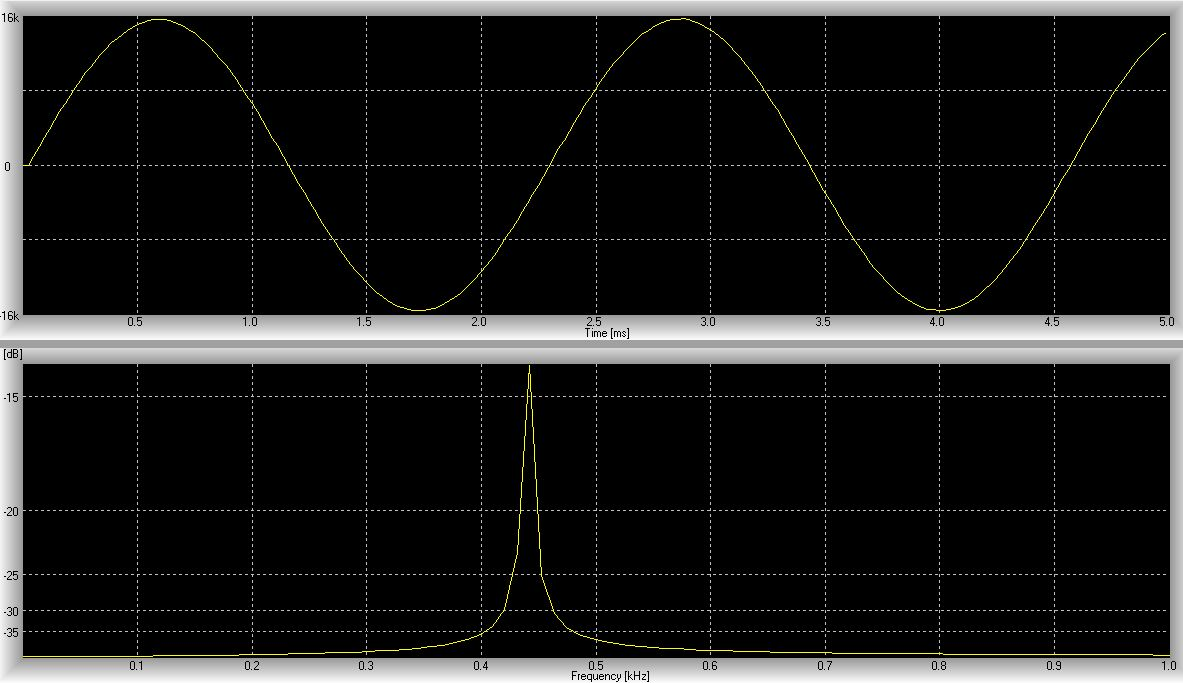
\includegraphics[scale=0.4]{Images/Sinus440Hz.JPG}
\caption[Verzeichniseintrag]{Sinusschwingung mit 440Hz }
\end{figure}
\begin{figure}[htb]
\centering
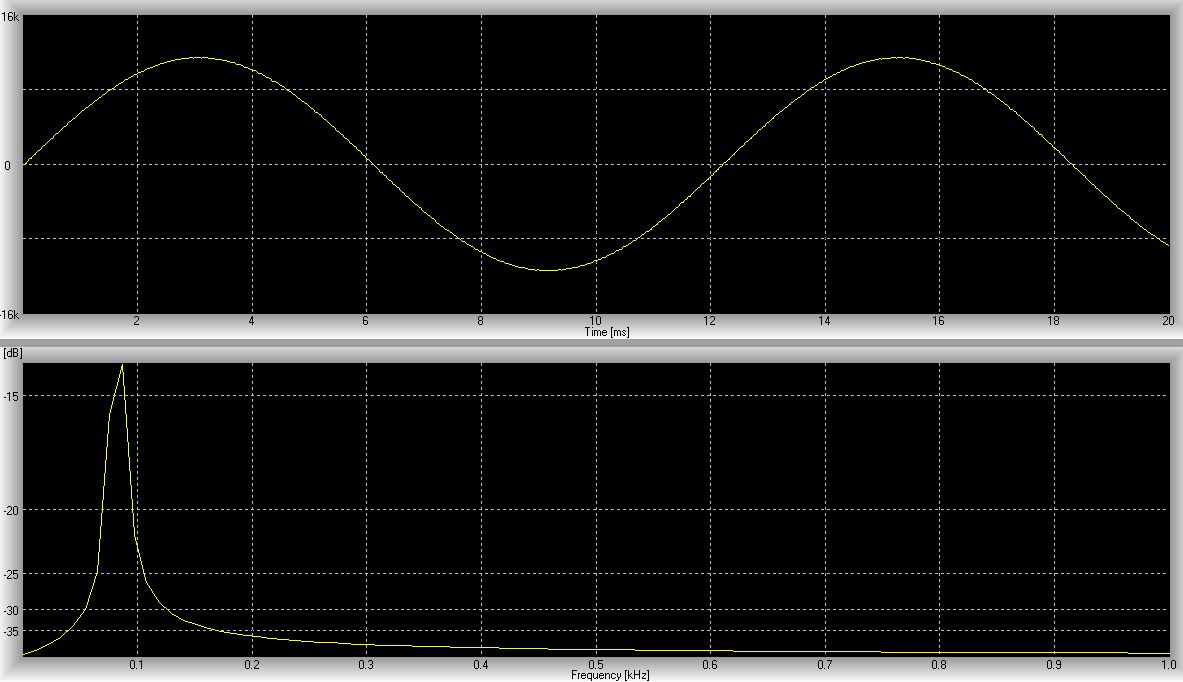
\includegraphics[scale=0.4]{Images/Sinus82Hz.JPG}
\caption[Verzeichniseintrag]{Sinusschwingung mit 82,406Hz }
\end{figure}

\subsection{Melodie}

Um eine Melodie zu erzeugen, müssen mehrere Töne nacheinnader und auch parallel
abgespeielt werden.


\end{document}
